%++++++++++++++++++++++++++++++++
\cscschapter{Cooperating Threads}
%++++++++++++++++++++++++++++++++

%%%%%%%%%%%%%%%%%%%%%%%%%%%%%%%%%%%%%%%%%%%%
\begin{frame}[fragile]{The Need Cooperation Between Threads}
%%%%%%%%%%%%%%%%%%%%%%%%%%%%%%%%%%%%%%%%%%%%
    \centering
    Most algorithms do not lend themselves to trivial parallelization like our \axpy example

%----------------------------
    \begin{code}{reductions : e.g. dot product}
        \begin{lstlisting}[style=boxcudatiny]
int dot(int *x, int *y, int n){
  int sum = 0.;
  for(auto i=0; i<n; ++i)
    sum += x[i]*y[i];
  return sum;
}
        \end{lstlisting}
    \end{code}
%----------------------------
\vspace{-7pt}
%----------------------------
        \begin{code}{scan : e.g. prefix sum}
            \begin{lstlisting}[style=boxcudatiny]
void prefix_sum(int *x, int n){
  for(auto i=1; i<n; ++i)
    x[i] += x[i-1];
}
        \end{lstlisting}
    \end{code}
%----------------------------
\vspace{-7pt}
%----------------------------
    \begin{code}{fusing piplined stencil loops : e.g. apply blur kernel twice}
        \begin{lstlisting}[style=boxcudatiny]
void twice_blur(float *in, float *out, int n){
  float buff[n];
  for(auto i=1; i<n-1; ++i)
    buff[i] = 0.25f*(in[i-1]+in[i+1]+2f*in[i]);
  for(auto i=2; i<n-2; ++i)
    out[i] = 0.25f*(buff[i-1]+buff[i+1]+2f*buff[i]);
}
        \end{lstlisting}
    \end{code}

\end{frame}

%%%%%%%%%%%%%%%%%%%%%%%%%%%%%%%%%%%%%%%%%%%%
\begin{frame}[fragile]{Block-Level Synchronization}
%%%%%%%%%%%%%%%%%%%%%%%%%%%%%%%%%%%%%%%%%%%%
    \begin{columns}[T]
        \begin{column}{0.3\textwidth}
            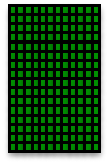
\includegraphics[width=\textwidth]{./images/smx.pdf}
        \end{column}

        \begin{column}{0.7\textwidth}
            CUDA provides mechanisms for cooperation between \emph{threads in a thread block}.
            \begin{itemize}
                \item All threads in a block run on the same SMX
                \item Resources for synchronization are at SMX level
                \item No synchronization between blocks
            \end{itemize}
        \end{column}
    \end{columns}

\end{frame}

%%%%%%%%%%%%%%%%%%%%%%%%%%%%%%%%%%%%%%%%%%%%
\begin{frame}[fragile]{Sharing Between Threads}
%%%%%%%%%%%%%%%%%%%%%%%%%%%%%%%%%%%%%%%%%%%%
    %\begin{info}{}
        Cooperation between threads requires sharing of results
        \begin{itemize}
            \item All threads in a block can share data via \emph{shared memory}
            \item Shared memory is extremely fast on-chip memory
            \begin{itemize}
                \item Much faster than performing transactions with global memory
                \item Can be used as a user-configured cache
            \end{itemize}
            \item Shared memory data is \emph{not visible} to threads in other thread blocks
        \end{itemize}
    %\end{info}

\end{frame}

%%%%%%%%%%%%%%%%%%%%%%%%%%%%%%%%%%%%%%%%%%%%
\begin{frame}[fragile]{Sharing Example : blur kernel}
%%%%%%%%%%%%%%%%%%%%%%%%%%%%%%%%%%%%%%%%%%%%
    $\text{out}_i \leftarrow 0.25\times(2\times\text{in}_i+\text{in}_{i-1}+\text{in}_{i+1})$
    \begin{info}{}
        \begin{itemize}
            \item each output value is a linear combination of neighbours in input array
            \item first we look at naiive implementation
        \end{itemize}
    \end{info}

    \begin{code}{Host implementation of blur kernel}
        \begin{lstlisting}[style=boxcudatiny]
void blur(double *in, double *out, int n){
  float buff[n];
  for(auto i=1; i<n-1; ++i)
    out[i] = 0.25*(2*in[i]+in[i-1]+in[i+1]);
}
        \end{lstlisting}
    \end{code}

\end{frame}

%%%%%%%%%%%%%%%%%%%%%%%%%%%%%%%%%%%%%%%%%%%%
\begin{frame}[fragile]{Blur kernel : no shared memory}
%%%%%%%%%%%%%%%%%%%%%%%%%%%%%%%%%%%%%%%%%%%%
    \begin{code}{Na\"ive implementation of blur kernel}
        \begin{lstlisting}[style=boxcudatiny]
__global__ void
blur(const double *in, double* out, int n) {
  int i = threadIdx.x + blockDim.x * blockIdx.x + 1;

  if(i<n-1) {
    out[i] = 0.25*(in[i-1] + 2*in[i] + in[i+1]);
  }
}
        \end{lstlisting}
    \end{code}

\end{frame}
